\onecolumn
\chapter{Auswertung}
\label{ch:auswertung}

\section*{Fehlerrechnung}
Für die statistische Auswertung von $n$ Messwerten $x_i$ werden folgende Größen definiert \cite{errorSkript25}:
\begin{align}
    \bar{x} &= \frac{1}{n} \sum_{i=1}^{n} x_i \vphantom{\sqrt{\sum_i^n}^2} && \text{\textcolor{gray}{Arithmetisches Mittel}} \label{eq:arithmetisches_mittel} \\
    \sigma^2 &= \frac{1}{n-1} \sum_{i=1}^{n} (x_i - \bar{x})^2 \vphantom{\sqrt{\sum_i^n}^2} && \text{\textcolor{gray}{Variation}} \label{eq:variation} \\
    \sigma &= \sqrt{\frac{1}{n-1} \sum_{i=1}^{n} (x_i - \bar{x})^2} \vphantom{\sqrt{\sum_i^n}^2} && \text{\textcolor{gray}{Standardabweichung}} \label{eq:standardabweichung} \\
    \Delta \bar{x} &= \frac{\sigma}{\sqrt{n}} = \sqrt{\frac{1}{n(n-1)} \sum_{i=1}^n(\bar x - x_i)^2} \vphantom{\sqrt{\sum_i^n}^2} && \text{\textcolor{gray}{Fehler des Mittelwerts}} \label{eq:fehler_mittelwert} \\
    \Delta f &= \sqrt{\left(\frac{\partial f}{\partial x} \Delta x\right)^2 + \left(\frac{\partial f}{\partial y} \Delta y\right)^2} \vphantom{\sqrt{\sum_i^n}^2} && \text{\textcolor{gray}{Gauß’sches Fehlerfortpflanzungsgesetz für $f(x,y)$}} \label{eq:gauss_fehlfortpflanzung} \\
    \Delta f &= \sqrt{(\Delta x)^2 + (\Delta y)^2} \vphantom{\sqrt{\sum_i^n}^2} && \text{\textcolor{gray}{Fehler für $f = x + y$}} \label{eq:fehler_summe} \\
    \Delta f &= |a| \Delta x \vphantom{\sqrt{\sum_i^n}^2} && \text{\textcolor{gray}{Fehler für $f = ax$}} \label{eq:fehler_proportional} \\
    \frac{\Delta f}{|f|} &= \sqrt{\left(\frac{\Delta x}{x}\right)^2 + \left(\frac{\Delta y}{y}\right)^2} \vphantom{\sqrt{\sum_i^n}^2} && \text{\textcolor{gray}{relativer Fehler für $f = xy$ oder $f = x/y$}} \label{eq:relativer_fehler} \\
    \sigma &= \frac{|a_{lit} - a_{gem}|}{\sqrt{\Delta a_{lit}^2 + \Delta a_{gem}^2}} \vphantom{\sqrt{\sum_i^n}^2} && \text{\textcolor{gray}{Berechnung der signifikanten Abweichung}} \label{eq:signifikante_abweichung}
\end{align}

\twocolumn


\section{Aufgabe 1: Verifizierung von Excel}
Wir wollen in der Auswertung damit beginnen, zu schauen, ob die Werte, die in dem vorgefertigtem Excel-Sheet bestimmt werden, stimmen. Dafür habe ich einmal ein 
eigenes Sheet erstellt, dass nochmal alle Werte erneut berechnet, hier habe ich jedoch die Formeln selbst per Hand eingertagen. Dies wurde dann für alle Tröpchen gemacht.
Excel und Python-Code für meine Auswertungen sind im GitHub \cite{githubPAP1} hinterlegt. Recht schnell war zu erkennen, dass alle Werte stimmen. 
Jedoch wollen wir auch wissen, ob Excel wirklich richtig rechnet, daher haben wir uns ein Tröpchen rausgesucht und werden seine eigenschaften per Hand berechen.
Ich habe mich dabei für das 9. Tröpchen entschieden. Hier sind seine Fall und Steigzeiten nochmal \hyperref[tab:testing]{tabellarisch (\ref*{tab:testing})} aufgelistet.
\begin{table}[b]
    \onecolumn
    \hspace*{-1.1cm}
    \centering
    \begin{tabular}{ c | c | c | c | c | c | c}
        \toprule
        $t_s \,  [s]$ & $t_f \,  [s]$ & $v_s \,  [m/s \cdot 10^{-5}]$ & $v_f \,  [m/s \cdot 10^{-5}]$ & $r_0 [m\cdot 10^{-7}]$ & $f_0 \cdot 10^-{1}$ & $q \, [C \cdot 10^{-19}]$ \\
        \midrule
        $13,9 \pm 0,3$ & $12,5 \pm 0,3$ & $4,01 \pm 0,14$ & $3,5935 \pm 0,1214$ & $5,86 \pm 0,10$ & $8,835 \pm 0,018$ & 1,514 \\
        $13,3 \pm 0,3$ & $12,1 \pm 0,3$ & $4,12 \pm 0,15$ & $3,761 \pm 0,130$ & $5,992 \pm 0,104$ & $8,858 \pm 0,018$ & 1,611 \\
        $13,4 \pm 0,3$ & $12,8 \pm 0,3$ & $3,89 \pm 0,14$ & $3,720 \pm 0,128$ & $5,959 \pm 0,103$ & $8,852 \pm 0,018$ & 1,547 \\
        $14,3 \pm 0,3$ & $14,4 \pm 0,3$ & $3,469 \pm 0,116$ & $3,502 \pm 0,117$ & $5,78 \pm 0,10$ & $8,821 \pm 0,018$ & 1,367 \\
        $13,7 \pm 0,3$ & $13,0 \pm 0,3$ & $3,844 \pm 0,134$ & $3,663 \pm 0,125$ & $5,9133 \pm 0,1017$ & $8,845 \pm 0,018$ & 1,512 \\
        \bottomrule
    \end{tabular}
    \label{tab:testing}
    \caption{Korrekturrechnung der Vorgegebenen Excel-Tabelle}
    \twocolumn
\end{table}

Dabei entspricht $t_s$ der gemessenen Steigzeit. Die Unsicherheit wurde auf $\Delta t_s = 0,3$ geschätzt, was in etwas die Reaktionszeit eines Menschen ist.
Die Ungenauigkeit der Stoppuhren ist angegeben gewesen mit $0,001s$. Diese kann jedoch entgen der Reaktionszeit und insbesondere der Messzeit vernachlässigt werden.
$t_f$ ist die gemessene Fallzeit. Sie hat denselben Fehler wie die Steigzeit. Die berechneten Geschwindigkeiten $v_f$ und $v_s$ sind dabei gleichnamig die Fall- und Steiggeschwindigkeit über $10Stk$. 
Dies entspricht einer Strecke von $0,0005m$. Die Unsicherheit der Geschwindigkeit wurde über die \hyperref[eq:gauss_fehlfortpflanzung]{Gauß'sche Fehlerfortpflanzung (\ref*{eq:gauss_fehlfortpflanzung})} bestimmt:
\begin{equation}
    \Delta v = \sqrt{\left(\frac{\Delta s}{t}\right)^2 + \left(\frac{v}{t} \cdot \Delta t\right)^2}.
\end{equation}

Hier haben wir für die Unsicherheit der Strecke $\Delta s = 0,000013m$ eingesetzt. Dies ist die Ungenauigkeit der Skala \cite{skript25}.

Die Berechnung des Radiuses ist der \hyperref[eq:radius]{Gleichung \ref*{eq:radius}} zu entnehmen. Wir wenden auf diese erneut die \hyperref[eq:gauss_fehlfortpflanzung]{Gauß'sche Fehlerfortpflanzung (\ref*{eq:gauss_fehlfortpflanzung})} an, um ihre Ungenauigkeit zu bestimmen und kommen damit auf die Gleichung:
\begin{equation}
    \frac{\Delta r}{r} = \sqrt{\left(\frac{\Delta v_f}{2v_f}\right)^2 + \left(\frac{\Delta \eta_0}{2 \eta_0}\right)^2 + \left(\frac{\Delta \rho}{2 \rho}\right)^2}
\end{equation}

Die Erdbeschleunigung $g$ wird dabei als >>unendlich<< genau angenommen und wird hier nicht berücksichtigt. Auch für $\eta_0$ ist keine Ungenauigkeit bekannt, weshalb diese in der Berechnugn auch als $0$ angenommen wurde. 

Die Ungenauigkeit des Korrekturthermes $\Delta f_0$ war ziemlich kompliziert zu berechnen, aber wurde zu
\begin{equation}
 \Delta f_0 = \frac{b}{(r p + b)^2} \sqrt{p^2 \Delta r^2 + r^2 \Delta p^2}
\end{equation}
berechnet. Der Ungenauigkeit von $q$ wird später noch besonderes Augenmerk zukommen, daher wird es in diesem Teil erstmal dabei gelassen.
Wir sehen, die Werte stimmen alle samt mit den von Excel überein.

\newpage

\section{Aufagabe 2: Histogramm}
Wir haben alle gemessenen Werte \hyperref[fig:hist_s]{histographisch \ref*{fig:hist_s}} aufbereitet. Die Bin-Breite beträgt dabei $0,2 \cdot 10^{-19} As$. Das Gesamtintervall geht von $0 As$ bis $10 \cdot 10^{-19} As$. 
\begin{figure}[h]
    \centering
    \includegraphics[width=0.45\textwidth, page=4 ]{Protokolle/\versuchsnummer/Chapter/Messprotokoll.pdf}
    \caption{Histogramm der betimmten Gesammtladung aller Messungen.}
    \label{fig:hist_s}
\end{figure}

Das Histogram ist später noch einmal \hyperref[fig:hist_b]{Ganzseitig (\ref*{fig:hist_b})} angeführt.
Auffällig ist, dass die Container nicht kontinuirlich sind und sich auch keine Gauskruve klar zeigen lässt.
Dies ist damit zu begründen, dass wir nicht nur einfach geladene Öl-Tröpfchen beobachtet haben. 
Im Gegenteil, wir haben sogar $6$-fach negativ geladene Öl-Tröpfchen beobachtet. Zumindest, wenn man den Rechnungen von Excel vertauen schenckt.
Hier ist also jedes >>Cluster<< zu verstehen als Sammlung der $n$-fach negativ geladenen Tröpchen.
Es lassen sich jedoch nicht klar 6 >>Cluster<< beobachten; wieso ist das so? Vermutlich liegt dies daran, dass das Ziel war, möglichst langsame Tröpchen zu beobachten, denn langsam steigene Tröpchen 
bedeuten physikalisch weniger stark geladene Tröpchen. Daher sind besonder die >>Cluster<< für $n= 1, 2, 3$ zu erkennen. Ab $n=4$ gibt es einen kruzen Peak und $n=5$ bzw. $n=6$ sind nicht mehr als >>Cluster<< zu erkennen.

\section{Aufgabe 3: Obergrenze}
In dem Excel-Sheet ist eine Obergrenze von $q_{1,max} =2,4C$ gesetzt (streng genommen $2,4 \cdot 10^{-19}C$, der Einfachheit, lassen wir den Potenzteil weg.). Dies bedeutet, dass jedes Teilchen mit einer Ladung von unter $q = 2,4C$ noch als einfach geladen gilt.
Aber wieso gerade $2,4C$? Dafür lohnt es sich den Literaturwert einmal anzusehen:
\begin{equation*}
    q_{lit} = e^- = 1,602 \cdot 10^{-19} C.
\end{equation*}

Dieser Wert sit alles andere als Willkürlich gewählt, der Wert ist das arithmetische Mittel von $e^-$ und $2e^-$. Dies ist in diesem Fall glecihbedeutent mit einer Abweichung von $50\%$.
Daher lässt sich dieser Wert als grundsätzlich vernünftig einschätzen. Aber als Optimal würde ich diesen Wert nicht einstufen. Eine ungenauigkeit von $50\%$ ist ziemlich groß.

Viel Eher halte ich einen Wert von $1,7$ oder $1,8$ für sinn voll. Damit wären nur noch Abweichungen von ca. $6\%$ bzw. $20\%$. 
Zur Viualisierung ist \hyperref[fig:plot_maxq]{Graph \ref*{fig:plot_maxq}}, welcher sehr schön die >>Cluster<< des Histogrammes wieder spiegelt,
dieses Mal als Platos. 

\begin{figure}[h]
    \centering
    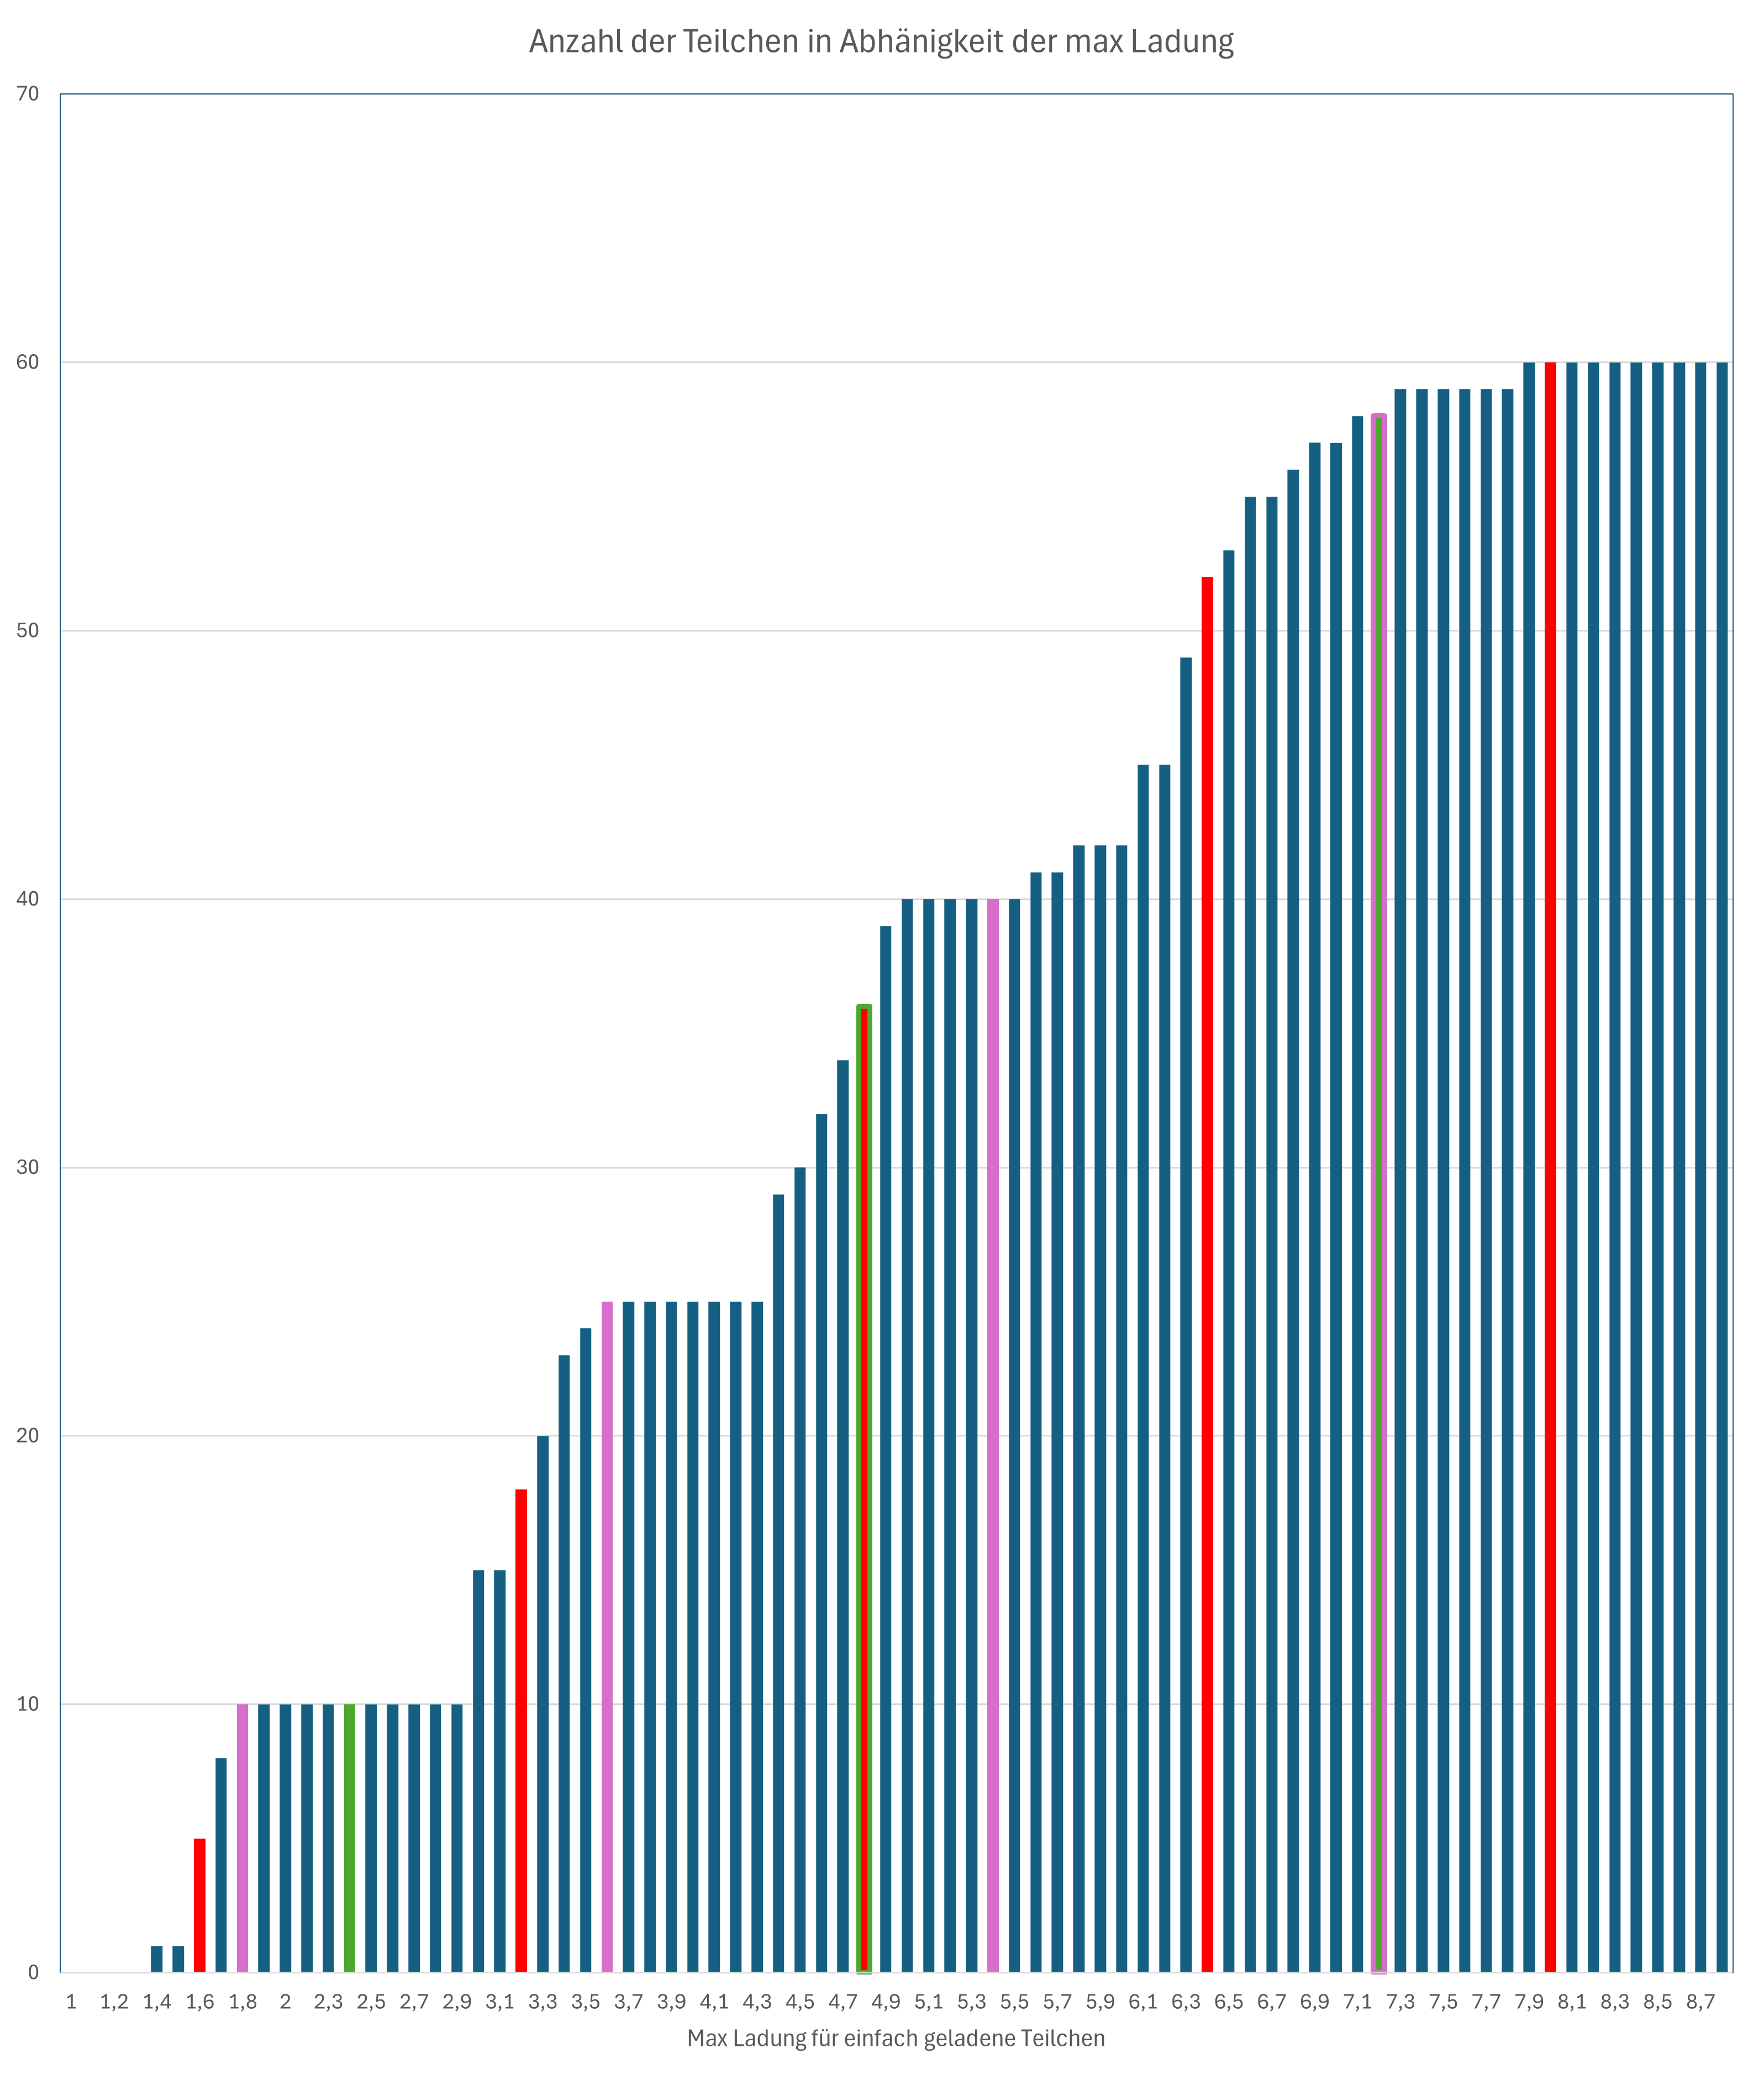
\includegraphics[width=0.37\textwidth]{img/22/Plot_MaxQ.png}
    \caption{Messungen vs. maximal Ladung für Einfachladung.}
    \label{fig:plot_maxq}
\end{figure}

Man sieht ganz schön, dass die roten Balken (ca. ein vielfaches der tatsächlichen Elementarladung) recht zu Beginn der Platos sthen.
Die grünen sind vielfache von $2,4$. Man sieht hier, dass diese eher zum ende der Platos sind, und insbesondere Platos überspringen. 
Daher scheinen die magenta farbenden die Sinnvollsten, denn diese liegen mittig auf den Platos. Diese sind die Balken, die ein vielfaches von $1,8$ darstellen. 
Auch dieser \hyperref[fig:plot_maxq_b]{Plot ist groß (\ref*{fig:plot_maxq_b})} später im Dokument zu finden.

Wir wollen unsere Messung nun also in zwei >>Teile<< aufteilen. Einmal in die Teilchen, die (vermutlich) einfach geladen sind, und die die zweifach geladen sind. 
Dies ist über unser Histogramm sehr gut möglich. Wir Wählen die zwei Intervalle $(1,0; 2,2)$ für einfach geladene Teilchen und $(2,6;3,8)$ für zweifach geladene Teilcehn.
Wir wollen insbesondere die \hyperref[eq:arithmetisches_mittel]{durchschnittliche Ladung (\ref*{eq:arithmetisches_mittel})} der zwei >>Cluster<< ermitteln und deren \hyperref[eq:fehler_mittelwert]{Fehler (\ref*{eq:fehler_mittelwert})}.
Dabei kommen wir auf folgende zwei Werte:
\begin{align}
    \overline{Q_1} = (1,58 \pm 0,04) \cdot 10^{-19}C \\
    \overline{Q_1} = (3,19 \pm 0,06) \cdot 10^{-19}C.
\end{align}

Wir brauchen nun noch die \hyperref[eq:standardabweichung]{Standardabweichungen (\ref*{eq:standardabweichung})}. Dann nehmen wir deren Maximal- bzw. Minimalwert. Dann wissen wir, dass sich ein Teilchen zu $99,7\%$ in der >>richtigen<< Umgebung befindet.
Somit kommen wir auf:
\begin{align}
    \text{obere Grenze für } 1e^- = 1,70 \cdot 10^{-19}C \\
    \text{untere Grenze für } 2e^- = 2,98 \cdot 10^{-19}C 
\end{align}

Damit ist es (fast) komplett ausgeschlossen, dass ein Wert über $1,8 \cdot 10^{-19}C$ kommt, wenn dieses Teilchen Einfachgeladen war. Über $2,4 \cdot 10^{-19}C$ sowieso erst nicht. Beide Werte wären valide, aber ersterer ist anatürlcih weitaus näher am realen Wert.

Das wir tatsächlich exakt eine Elementarladung in den Tröpfchen haben, ist nicht garantierbar über diesen Verscuh, aber wahrscheinlich ist dies dennoch. 
Denn wir haben aktiv versucht die langsamsten Teilchen zu beobachten, und selbst dabei einige Teilchen mit 2-, 3- oder noch Mehr-Fachladung gemessen. Und kein einziges Teilchen.
Ein wichtes ABER ist jedoch, dass wir einen Messwert haben, der nicht in der $3\sigma$-Umgebung der einfachen Elementarladung liegt. Besagter Wert liegt bei $1,367 \cdot 10^{-19}C$. 
Dieser Wert stellt damit eine absolute Ausnahme dar, aber schließt damit nicht pauschal aus, dass wir ggf. doch eine kleinere Minimalladung haben. Wahrscheinlich ist jedoch wie angemerkt, dass es sich um eine stochhastische Besonderheit handelt, aber (offensichtlich) im Rahmen des Möglichen leigt. 

\section{Aufgabe 4: Systemischer Ladungsfehler}
Als nächstes wollen wir uns die Berechnung der Ladung anschauen, welche über die \hyperref[eq:ladung]{Gleichung \ref*{eq:ladung}} berechnet haben. Insbesondere wollen wir ihre Ungenauigkeit nach der \hyperref[eq:gauss_fehlfortpflanzung]{Gauß'sche Fehlerfortpflanzung (\ref*{eq:gauss_fehlfortpflanzung})} betrachten. 
Die Gleichung ist im Skript bereits vorgegeben \cite{skript25}:

\begin{equation}
    \frac{\Delta q}{q} =
    \sqrt{
        \begin{array}{l}
            \left( \tfrac{3 \,\Delta s}{2s} \right)^{2}
            + \left( \tfrac{\Delta \rho}{2\rho} \right)^{2}
            + \left( \tfrac{3 \,\Delta \eta}{2\eta} \right)^{2} \\[6pt]
            + \left( \tfrac{\Delta d}{d} \right)^{2}
            + \left( \tfrac{\Delta U}{U} \right)^{2}
        \end{array}
    }
    \label{eq:fehler_q}
\end{equation}

Zunächst wollen wir verstehen, woher die Faktoren in den verschiedenen Quotienten kommen. Dafür lohnt es sich nochmal \hyperref[eq:ladung]{Gleichung \ref*{eq:ladung}} genau anzusehen. Denn für die Gau'sche Fehlerfortpflanzung müssen wir nach allen Feherquellen partiel ableiten. 
Kennt man die Ableitungsreglen, muss man sich nur noch die proportionalität der einzelnen Variablen anschauen und sieht, dass die Strecke $s$ nur indirekt in den Geschwindigkeiten steckt. Fasst man alles sinn voll zusamen, so kommt man zur Proportionalitöät $q \propto \sqrt{s^3}$, dies wird zum Faktor $\frac{3}{2}$.
Beim Druck ist es ähnlich, dieser geht via $q \propto \sqrt{p}$ in die Gleichung ein, woraus sich der Faktor $\frac{1}{2}$ bildet.
Das $\eta$ steht sowieso schon in der dritten Potenz unter der Wurzel, also $q \propto \sqrt{\eta 3}$ was zu einem Faktor $\frac{3}{2}$ führt.
Negative Vorzeichen können ignoriert werden, da alles quadriert wird. $d$ und $U$ gehen dabei linear in die Gleichung ein und haben daher eine Koeffizienten. 

Nun berechnen wir hier die systemische Ungenauigkeit nach Gauß, so kommen wir insegsamt auf eine Ladung von:
\begin{equation}
    \underline{e^- = (1,58 \pm 0,08) \cdot 10^{-19}C}.
\end{equation}

Für die Berechnung wurden folgende Werte benutzt:
\begin{table}
    \centering
    \begin{tabular}{c | c | c}
        \toprule
        Größe & Wert & Abweichung \\
        \hline
        s [m] & 0,000500 & 0,000013 \\
        p [Pa] & 100710,00 &  0,10 \\ 
        d [m] & 0,006 & 0,00005 \\
        U [V] & 500,0 & 2,5 \\
        \bottomrule
    \end{tabular}
    \caption{Eingesetzte Größen zur Bestimmung der systemischen Ungenauigkeit nach Gleichung \ref*{eq:fehler_q}.}
\end{table}

und zu letzt:
\begin{equation}
    \frac{\Delta \eta}{\eta} = 0,02.
\end{equation}

\section{Aufgabe 5: Statistischer Fehler}
Wir wollen uns nun auf die entstandenen statistischen Fehler konzentrieren und insbesondere auch diese mit den Excel-Werten vergleichen.
Wir nehmen dieselben 5 Messungen eines Tröpchens wie in \hyperref[tab:testing]{Tabelle \ref*{tab:testing}}. Dieses Mal wollen wir uns - wie angekündigt - um die Ungenauigkeit der Ladungsbestimmung kümmern.
Zunächst gehen wir dabei nur davon aus, dss statistische Fehler in der Geschwindigkeitsmessung entstanden sind, dies bedeutet insbesondere, dass wir die statistischen Fehler des Zeitstoppens berücksichtigen müssen.
Wir rufen uns in Erinnerung, dass die Werte via \hyperref[eq:ladung]{Gleichung \ref*{eq:ladung}} berechnet wurden. Wir rufen uns unsere Werte erneut in Erinnerung und berechnen Ihren durchschnitt:
\begin{align}
    q_1 = 1,514 \, [C \cdot 10^{-19}] \notag \\
    q_2 = 1,611 \, [C \cdot 10^{-19}] \notag \\
    q_3 = 1,547 \, [C \cdot 10^{-19}] \notag \\
    q_4 = 1,367 \, [C \cdot 10^{-19}] \notag \\
    q_5 = 1,512 \, [C \cdot 10^{-19}] \notag \\
    \overline{q} = 1,510 \, [C \cdot 10^{-19}]
\end{align}

Wir kommen dabei auf eine Standardabweichung der Einzelmessung von
\begin{equation}
    \sigma = 0,089 
\end{equation}
und auf eine Standardabweichung des Mittelwertes von
\begin{equation}
    \Delta \overline{q} = 0,040.
\end{equation}

Diese sind nicht mit den von Excel berechneten Werten konsistent. Die Abweichung der Standardabweichung der Einzelwerte, die von Excel berechnet wurde, ist 9\% größer.
Die Standardabweichung des Mittelwertes ist hingegen nur 30\% des Wertes, von den hier berechneten Werten. Die Abweichungen kommen sehr wahrscheinlich daher, dass hier lediglich 5 Tropfen zur ebrechnung dienten, 
in der Excel Tabelle jedoch 60 Werte. Die statistische Genauigkeit der Werte geht $\propto \frac{1}{\sqrt{n}}$. Somit werden die Werte genauer, wenn es mehr werden.
Zudem haben wir den Wert $q_4$, welcher eine besonderes hohe Abweichung hat und das Ergebnis nennenswert verändert. 
Ein weiterer Grund dürfte sein, dass hier in der Rechnung das Tröpchen immer dieselbe Ladung trug, während es in der Excel Tabelle $1-5$ Ladungen sein können. 
Wir rechnen denncoh mit dem hier berechneten Wert weiter,
und brechnen nun den \hyperref[eq:fehler_mittelwert]{Fehler des Mittelwertes (\ref*{eq:fehler_mittelwert})} und kommen dabei auf einen Wert:
\begin{equation}
    \underline{\Delta_{stat} q = 0,04 \, [C \cdot 10^{-19}]}.
\end{equation}


\subsection*{Gesamterfehler von q}
Wir haben somit den statistischen und den systematischen Fehler bestimmt. Wir wollen aber die Gesamtzungenauigkeit haben, daher werden die Fehler gemäß \hyperref[eq:fehler_summe]{Gelcihung \ref*{eq:fehler_summe}} verrechnet zu:
\begin{equation}
    \Delta_{ges} q = \Delta e^- = \sqrt{(\Delta_{sys} q)^2 + (\Delta_{stat} q)^2}.
\end{equation}
Ausgerechnet ist es dann:
\begin{equation}
    \underline{\Delta e^- = 0,09 \, C \cdot 10^{-19}.}
\end{equation}

Wir kommen final auf ein Ergebnis von 
\begin{equation}
    \boxed{q = e^- = (1,58 \pm 0,09) \, C \cdot 10^{-19}}.
\end{equation}

\section{Aufgabe 6: Signifikanz bestimmen}
in der letzten Aufgabe wollen wir nochmal schauen, wie weit unser Wert vom Literaturwert $e^-_{lit} = 1,602 \, C \cdot 10^{-19}$ abweicht. Wir berechnen die \hyperref[eq:signifikante_abweichung]{Signifikanz (\ref*{eq:signifikante_abweichung})} und kommen auf ein Ergebnis von:
\begin{equation}
    \boxed{\frac{\left| 1,602 - 1,580 \right|}{0,09} = 0,24\sigma}
\end{equation}

\onecolumn
\begin{figure}
    \centering
    \hspace*{-2.2cm}
    \includegraphics[width=1.3\textwidth, page=4 ]{Protokolle/\versuchsnummer/Chapter/Messprotokoll.pdf}
    \caption{Histogramm der betimmten Gesammtladung aller Messungen.}
    \label{fig:hist_b}
\end{figure}
\twocolumn
\onecolumn
\begin{figure}[h]
    \centering
    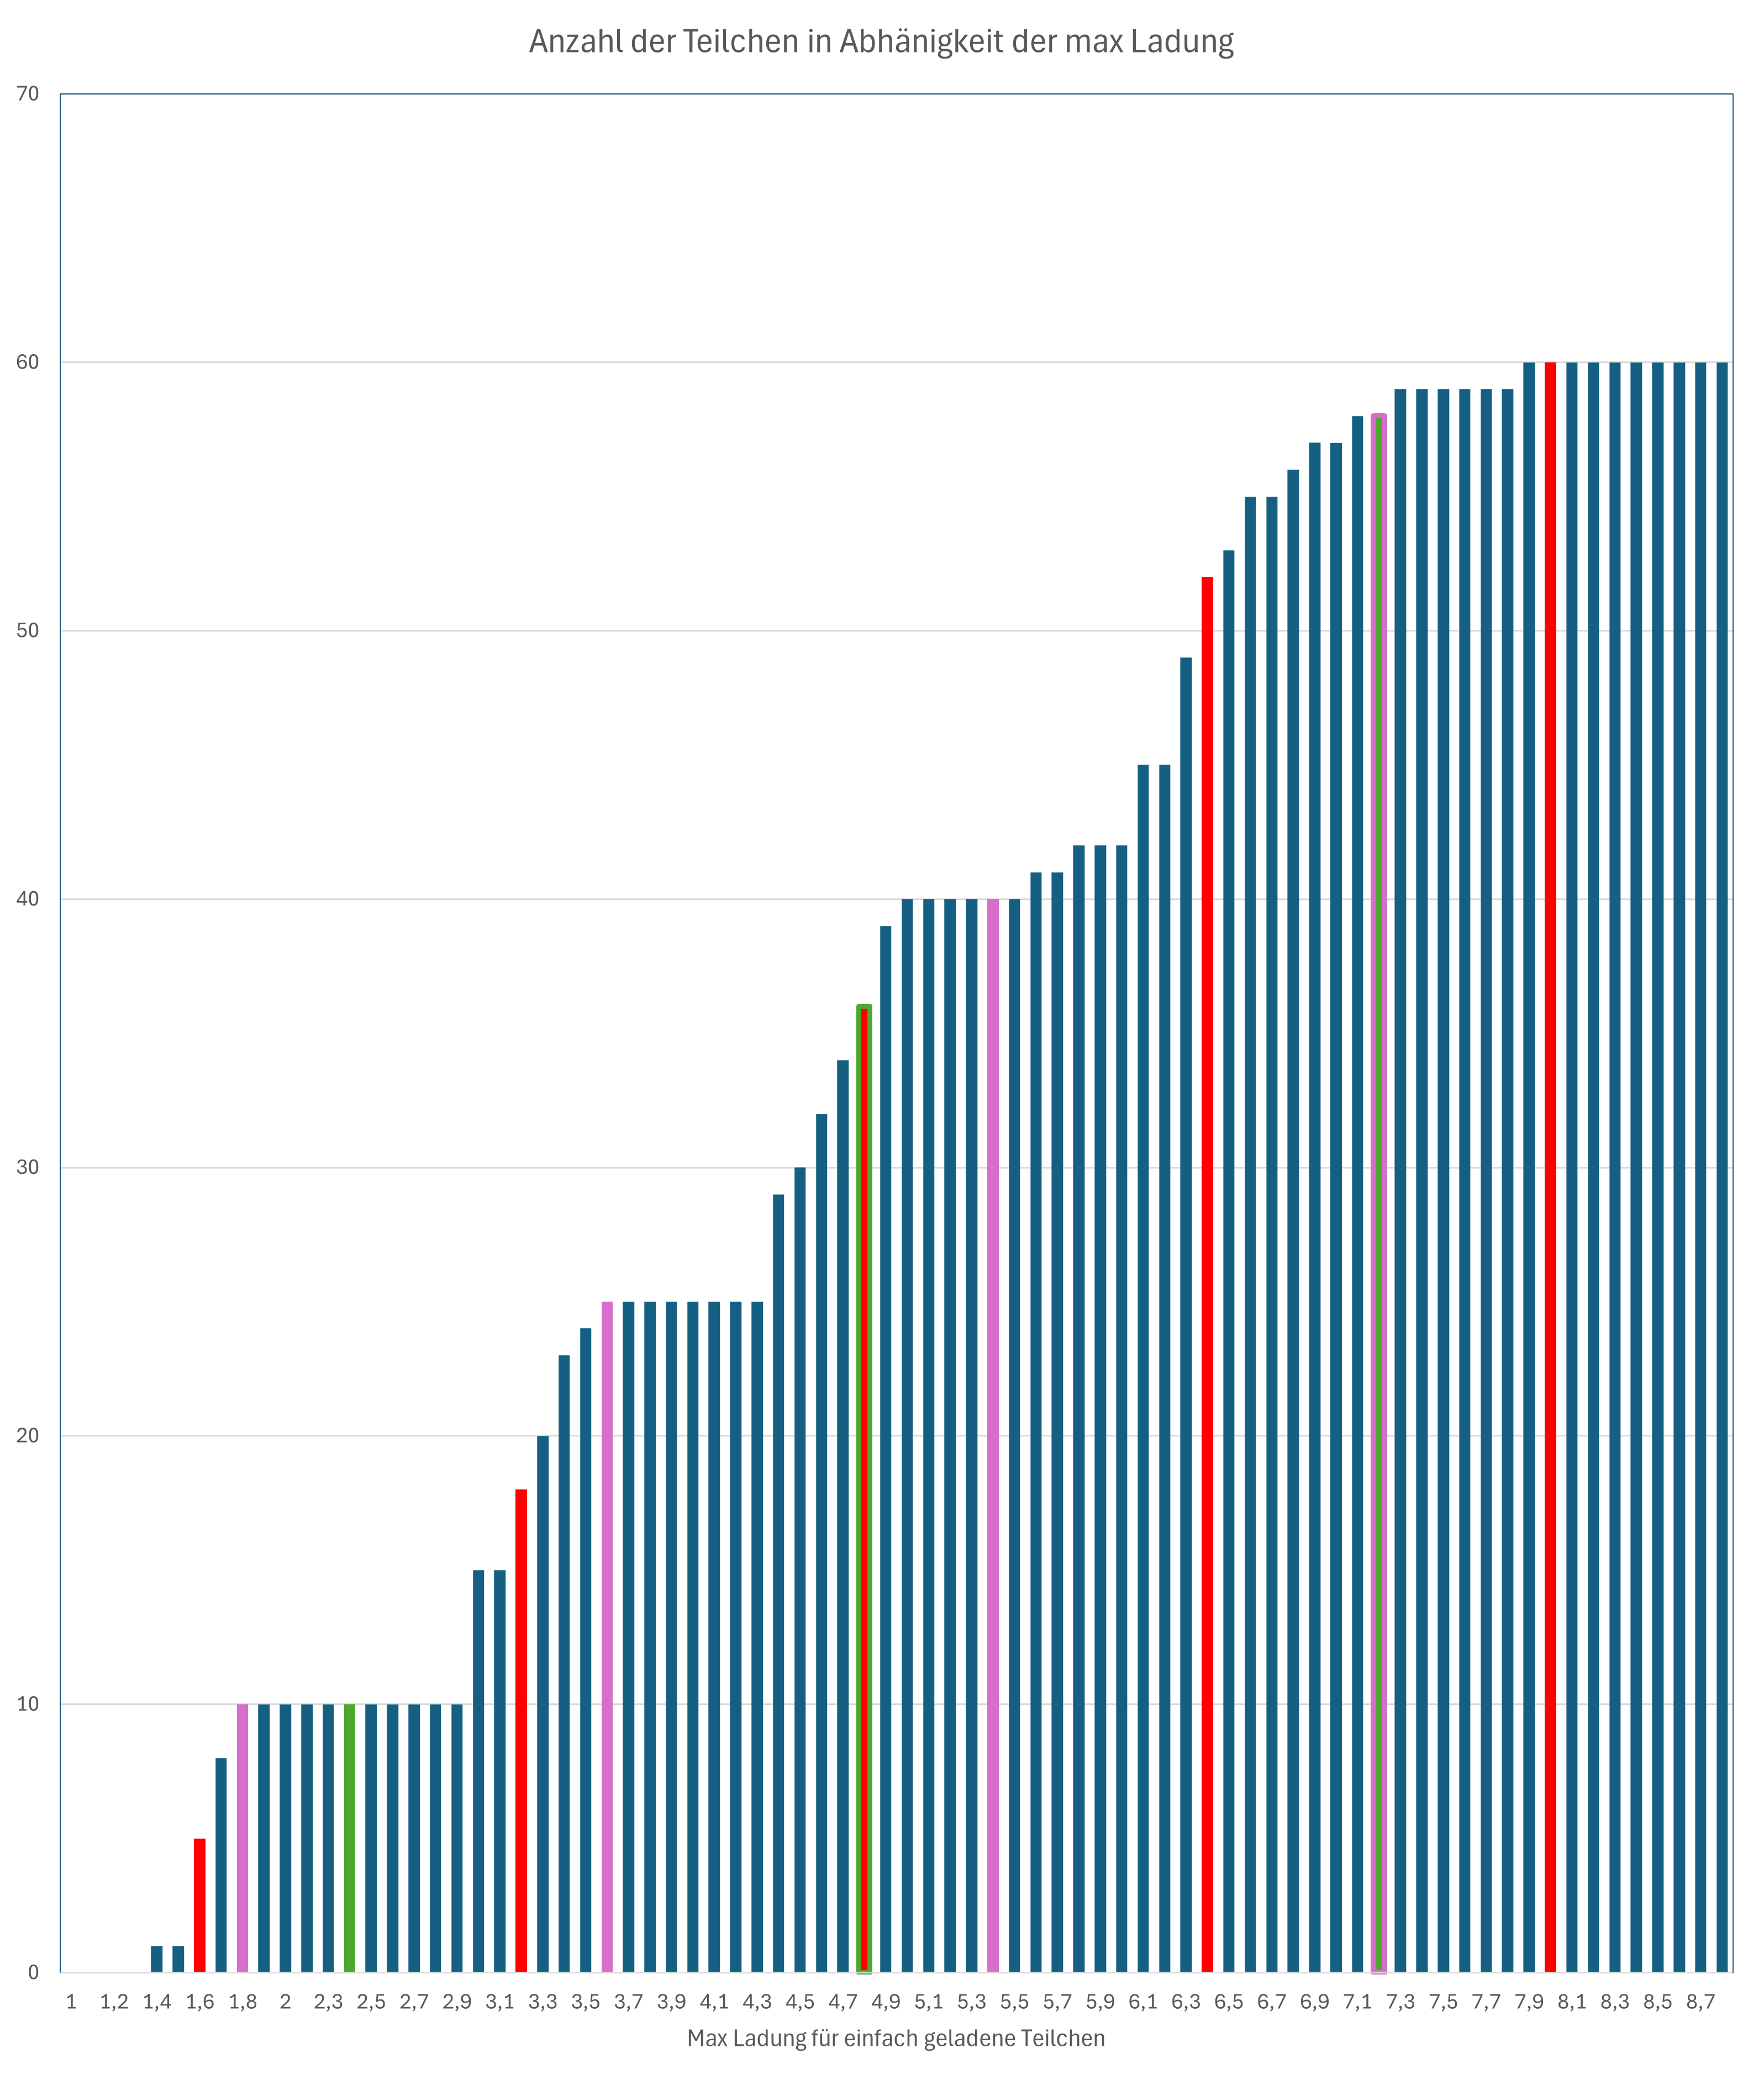
\includegraphics[width=\textwidth]{img/22/Plot_MaxQ.png}
    \caption{Messungen vs. maximal Ladung für Einfachladung. Rot sind vielfache von $1,6$, magenta von $1,8$ und grün von $2,4$.}
    \label{fig:plot_maxq_b}
\end{figure}
\twocolumn
